\chapter{User Interface}


\section{Design}
Das Projekt erhält eine möglichst einfach gehaltene Benutzeroberfläche. Durch die farbliche Trennung von Funktionen und fixen Bereichen für die Daten, soll die Oberfläche einfach und Intuitiv gestaltet werden. Zusätzlich wird die Oberfläche Responsive gestaltet, damit die Oberfläche an alle Geräte angepasst wird.

Es wurden Mock-ups anhand von einfachen Handskizzen erstellt, um das aussehen und die Funktionen der Benutzeroberfläche zu planen.

\section{Ansichten}
\subsection{Startseite}
\begin{figure} [H]
	\begin{center}
	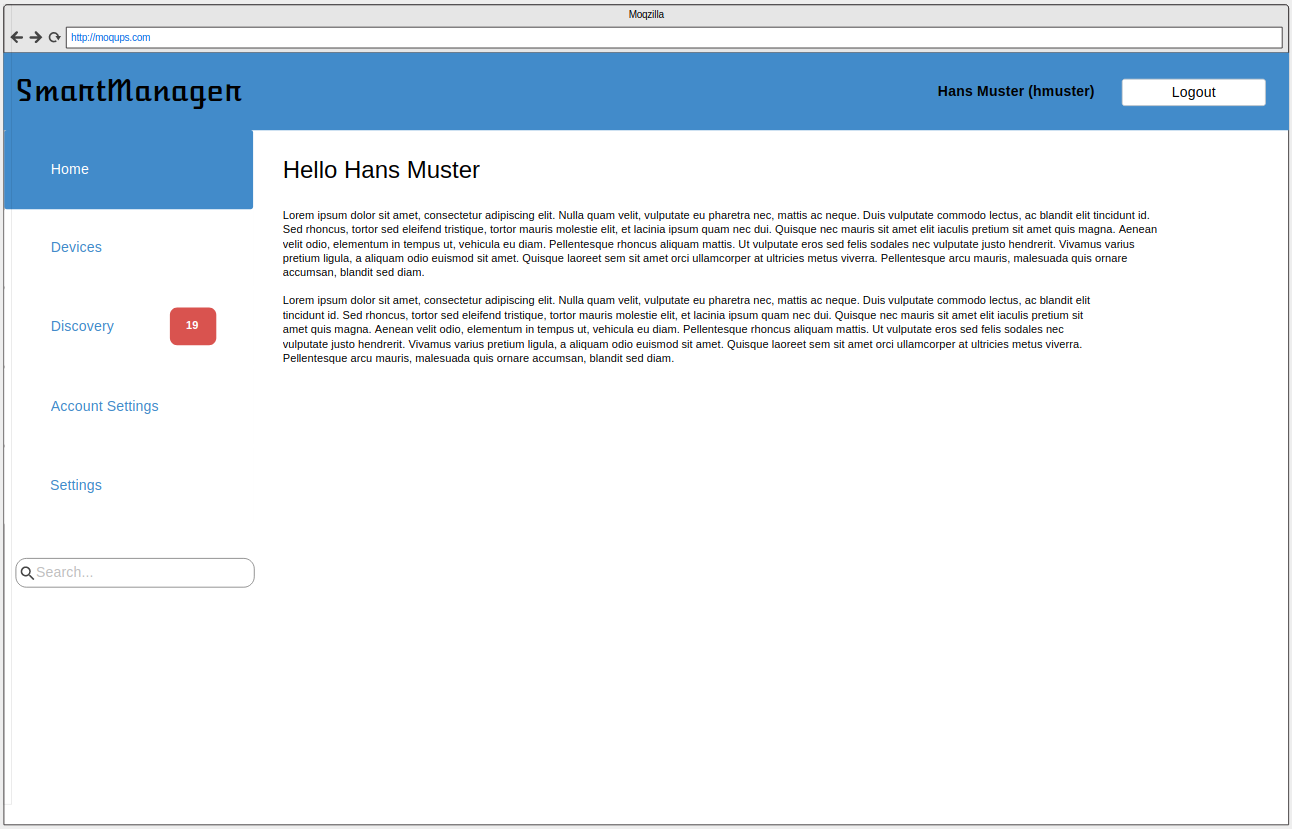
\includegraphics[width=0.80\textwidth]{images/home.png}
	\caption{Startseite}
	\end{center}
\end{figure}
Die Startseite zeigt dem Benutzer Hilfestellungen an und führt den Benutzer durch die ersten Schritte. Auf der Linken Seite befindet sich das Menu und eine Suche. Oben Rechts findet der Benutzer den Loginbereich und die Benutzerangaben.

Beim Menu gibt es statische, sowie dynamische Einträge. Der Discoveryeintrag ist ein dynamischer Eintrag und zeigt die Anzahl gefundenen Geräte an.

\subsection{Device List}
\begin{figure} [H]
	\begin{center}
	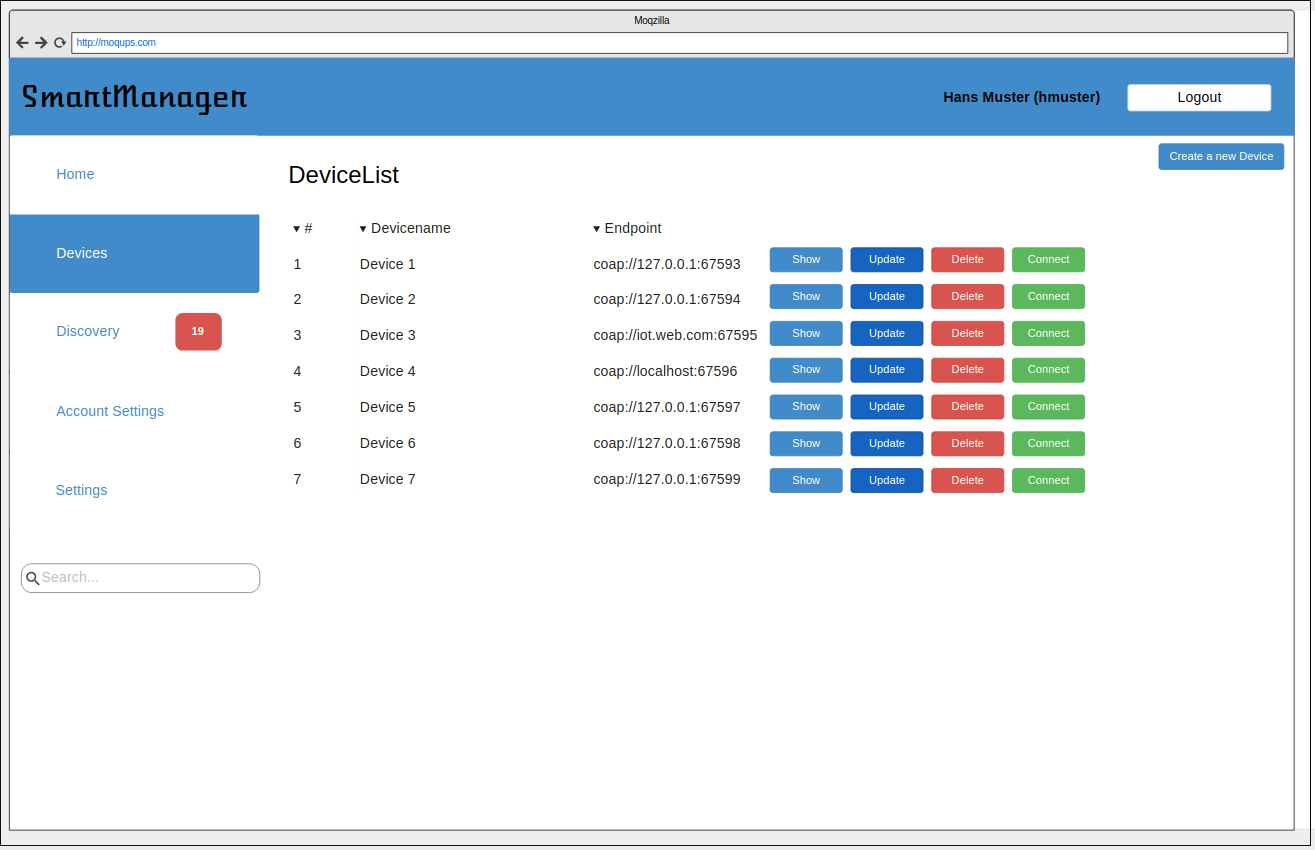
\includegraphics[width=0.80\textwidth]{images/devicelist.png}
	\caption{Device List}
	\end{center}
\end{figure}
In der Device Liste werden alle Devices angezeigt. Dazu wird zu jedem Device die jeweiligen Möglichkeiten als Button eingeblendet. So kann man ein Device betrachten, Anpassen, Löschen und sich mit dem Gerät verbinden. Zusätzlich werden die Daten, wie zum Beispiel Endpoint angezeigt.

Oben rechts befindet sich der Button, um weitere Devices zu erstellen.
\subsubsection{Buttons}
\begin{description}
\item [Show] Zeigt die Details zu einem Device an
\item [Update] Führt zum Device Update Formular, damit das Device angepasst werden kann.
\item [Delete] Button, der das Device aus der Applikation löscht
\item [Connect] Button, um sich mit dem Gerät zu verbinden.
\item [Create a new Device] Führt zur Create Device Ansicht.
\end{description}


\subsection{Create Device}
\begin{figure} [H]
	\begin{center}
	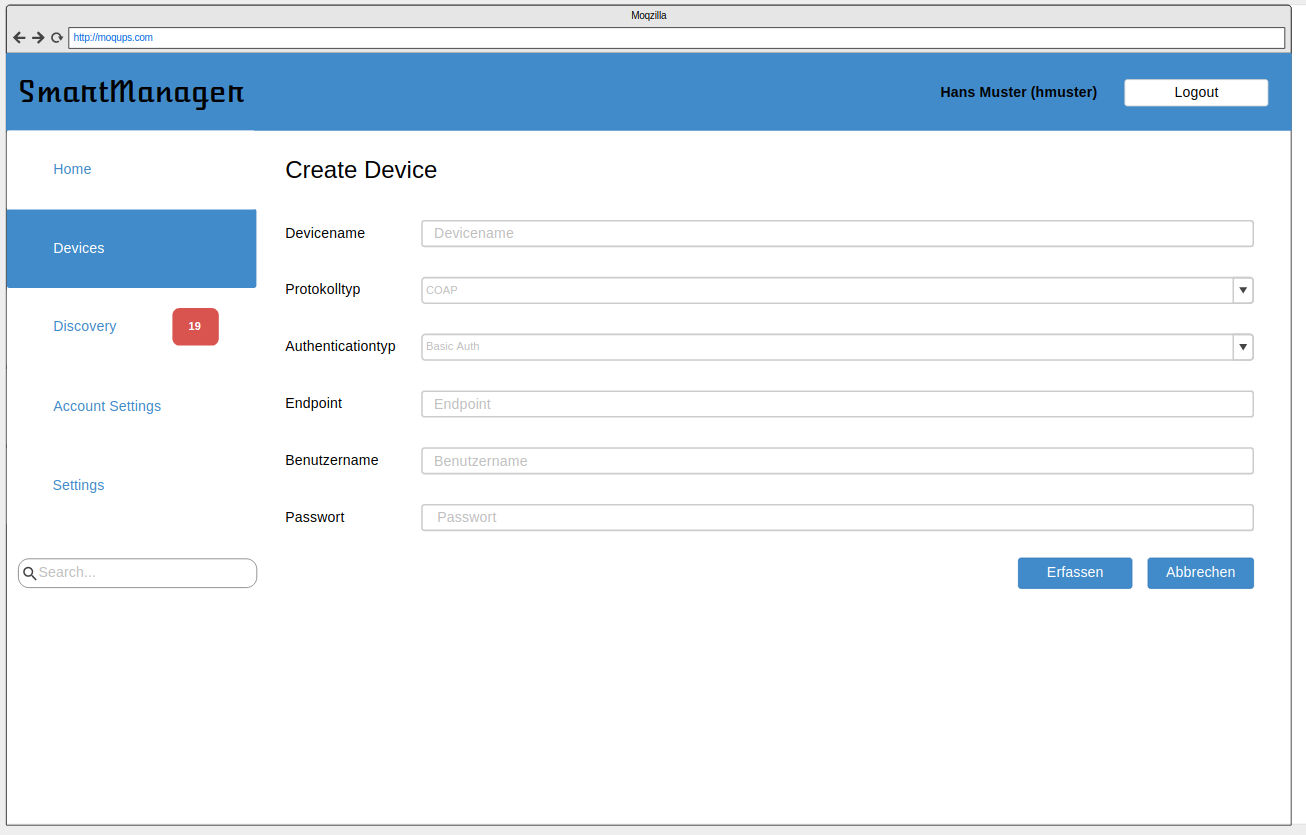
\includegraphics[width=0.80\textwidth]{images/createdevice.png}
	\caption{Create Device}
	\end{center}
\end{figure}
Bei der Create Device Ansicht kann ein neues Device erstellt werden. Dadurch wird das Device manuell erfasst und in der Datenbank abgelegt. Dies kann gemacht werden, wenn das Device nicht via Discovery gefunden worden ist.

Je nach Combobox Auswahl passt sich das Formular an, um zum Beispiel auch Zertifikate hinterlegen zu können.

\subsubsection{Buttons}
\begin{description}
\item [Erfassen / Update] Erstellt oder passt ein Device an
\item [Abbrechen] Bricht den Device Create ab und führt zur Device List Ansicht
\end{description}

\subsection{Device Details}
\begin{figure} [H]
	\begin{center}
	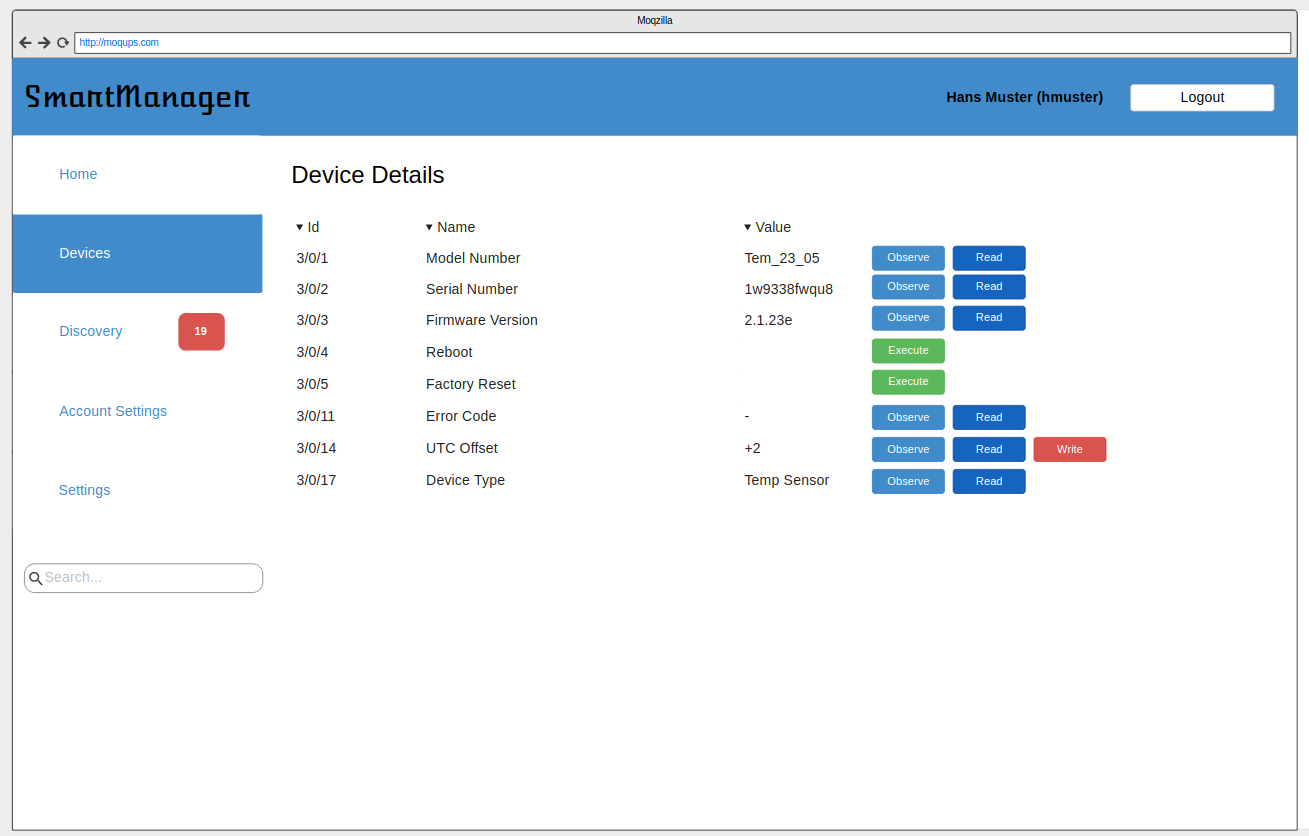
\includegraphics[width=0.80\textwidth]{images/devicedetails.png}
	\caption{Device Details}
	\end{center}
\end{figure}
Alle wichtige Informationen eines Devices werden in dieser Übersicht angezeigt. Zu Jeder Ressource wird die Id, der Name und den aktuellen Wert angezeigt. Je nach Ressource passen sich die Möglichen Aktionen an. Dabei gibt es Observe, Read, Write und Execute. Bei Write wird ein zusätzliches Eingabefeld eingeblendet, um den gewünschten Wert eintragen zu können.


\subsubsection{Buttons}
\begin{description}
\item [Observe] Startet ein Observer für die gewünschte Ressource.
\item [Read] Liest die Ressource vom Device
\item [Write] Schreibt den Wert in die Ressource und aktualisiert den Eintrag in der Datenbank
\item [Execute] Führt einen Befehl auf dem Device aus
\end{description}

\subsection{Discover Device}
\begin{figure} [H]
	\begin{center}
	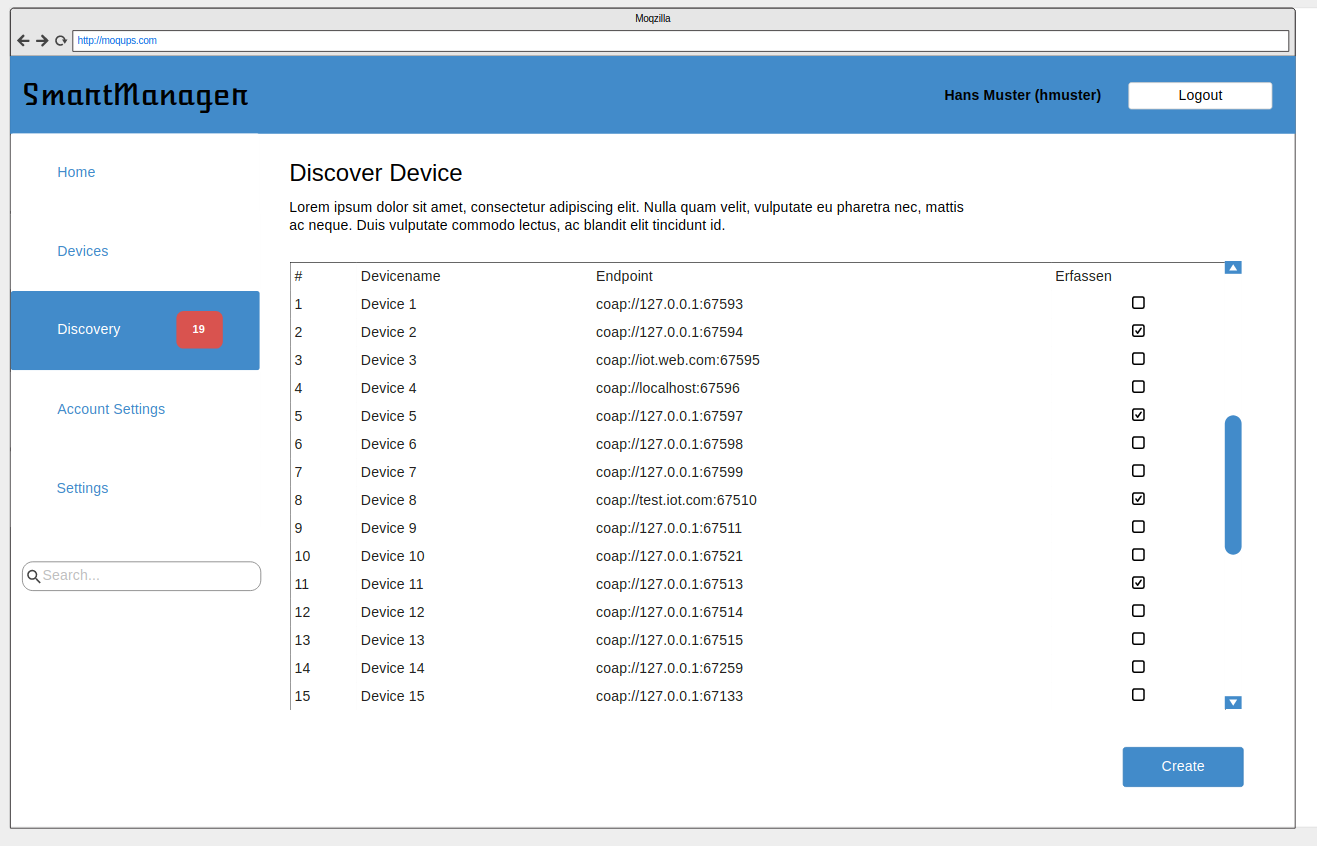
\includegraphics[width=0.80\textwidth]{images/devicediscover.png}
	\caption{Device Details}
	\end{center}
\end{figure}
Alle durch das Discovery gefundenen Devices werden in dieser Übersicht aufgelistet. Dazu werden direkt die wichtigen Daten angezeigt und man hat die Möglichkeit das gewünschte Device zur Applikation hinzuzufügen. Die Anzahl gefundenen Devices werden auf der Linken Seite im Menu angezeigt und passt sich dynamisch an.

\subsubsection{Buttons}
\begin{description}
\item [Create] Erstellt für die ausgewählten Devices ein Deviceobjektauf der Datenbank
\end{description}

